\documentclass[Preamble]{subfiles}
\begin{document}

\chapter{Domain Name System}


Domain Name System, DNS, is used to find IP-addresses from a logical name using the concept of the Host Lookup Table.
The Host Lookup Table, HLT, was a file placed on every computer connected to the network which contained the IP-address and the logical name for each computer connected\cite[History section]{wiki-hosts}.

When the HLT was updated, all computers needed to add the address which, due to the expansion of connecting computers to the network, became an obstacle and hindrance for the flow.
To solve this the DNS system was invented in 1982\cite[History section]{wiki-dns}.

DNS is like a big telephone book which everyone uses to lookup IP-addresses from logical names, through an address record (A record)\cite[p. 210]{Tanenbaum}, rather than everyone keeping track of all connected addresses.



\section{DNS fundamentals}
To find the computer's host name the command \code{hostname} will show the logical human readable name for the computer. 
The hostname will be shown on the list of connected computers on a  network.
\\
\\
In Linux the command \code{nm-tool} will access the NetworkManager Tool and among others, show the IP-address, MAC-address, connection state and DNS-server for the computer.
This is shown in Figure \ref{fig:nm-tool}\footnote{Note that this is on a virtual machine which do not show as much as a native Linux machine will}.
\\
You can run a similar command in Windows; \code{ipconfig /all} to access IP-address, DNS-server, MAC-Address ect. shown in Figure \ref{fig:ipconfig}.


\begin{figure}[H]
\centering
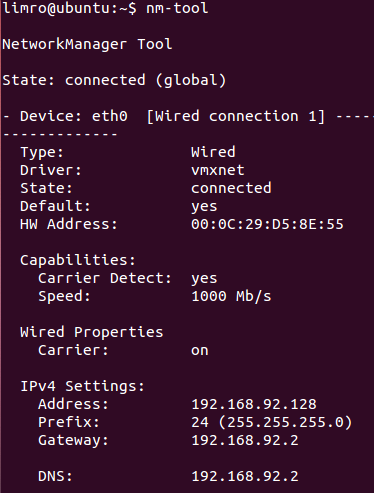
\includegraphics[scale=0.7]{nm-tool.png}
\caption{Use of the command \code{nm-tool}}
\label{fig:nm-tool}
\end{figure}

\begin{figure}[H]
\centering
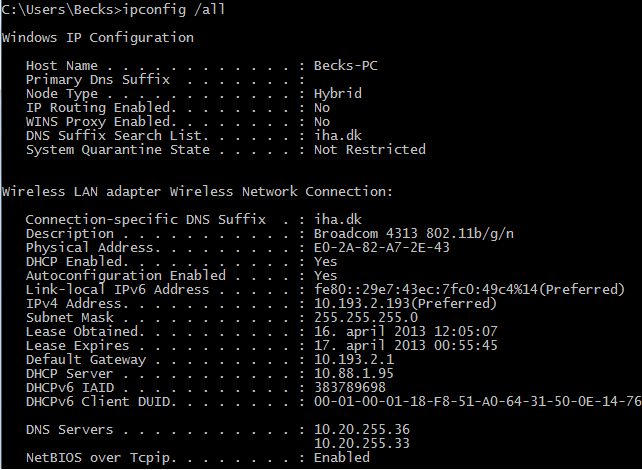
\includegraphics[scale=0.7]{ipconfig.png}
\caption{Use of the command \code{ipconfig /all}}
\label{fig:ipconfig}
\end{figure}

To detect an IP-address and determine the latency to the server use the \code{ping} command.
\code{ping} will target either a webserver name to get the IP-address or target the IP-address directly without asking the DNS-server.
This is shown on figure \ref{fig:ping}


\begin{figure}[H]
\centering
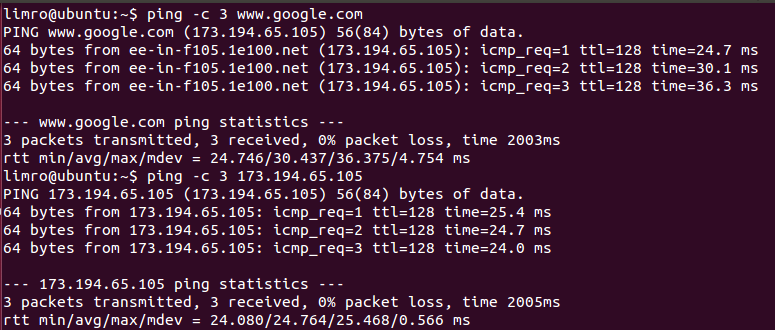
\includegraphics[scale=0.7]{ping}
\caption{Use of the command \code{ping -c 3 www.google.com}}
\label{fig:ping}
\end{figure}


Before makeing a lookup at the DNS server the system will check local HLT file, located in  \textit{/etc/hosts}, to see if any redirects or A records are listed.
Redirections are created by typing the static IP-address followed by the new logical name as shown in Code snippet \ref{lst:redirect}


\begin{lstlisting}[caption={Hosts file redirection}, style=Code-Bash, label=lst:redirect]
# Redirections
212.130.55.139 vejr #Resolve vejr to "www.dmi.dk"
159.20.6.38 nyhed #Resolve nyhed to "www.dr.dk"
157.55.46.241 mail #Resolve mail to "www.hotmail.com"
\end{lstlisting}

\vspace{10px}

When requesting a webserver through a DNS, the root servers first redirect to the top-level domain server, TLD, which contains the '.com', '.net', '.dk' etc \cite[p. 192]{Tanenbaum}.
From here the domain server can return the IP-address for the name server to which the client can connect. 
This will then (most likely) recursively or (less likely) iterative\footnote{See section \ref{sec:nameRes}, Name resolution} return the specified IP-address to the client.
\\
\\
Each DNS server is responsible for looking up domains in nonoverlapping parts called 'zones'. 
A zone is implemented by a separate name server\cite[p. 202-205]{Tanenbaum}.
\\
\\
When looking for a host name there can be multiple units with the same logical name. 
However it is possible to specify a name for a unit to unambiguously unique with a '.' (dot) at the end of the logical address which is called a fully qualified domain name (FQDN)\cite{wiki-fqdn}.
\\
Multiple computers could have the name \textit{myComputer} but if looking for a computer on a network called \textit{work.net.} there can only be one computer with the name \textit{myComputer.work.net.}



\newpage
\section{Name resolution}\label{sec:nameRes}

When looking up an IP-address it can be resolved in two different ways.
In iterative name resolution the root DNS server return the IP-address for the a DNS server which contains information of the requested country code. 
Afterwards the client will ask this DNS server for the IP-address and so on until the client the requested IP-address.
This DNS query/response transaction type of resolution requires the client involvement for each request to a DNS server which leads to lower performance cost for the DNS servers \cite[p. 205-209]{Tanenbaum}.

\begin{figure}[H]
\centering
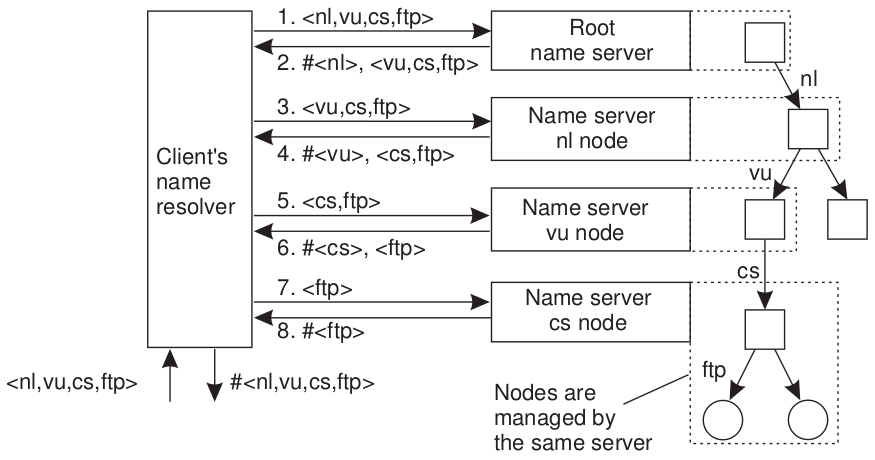
\includegraphics[scale=0.6]{iterativ}
\caption{Iterative request for an IP-address}
\label{fig:iterativ}
\end{figure}


In recursive name resolution the root DNS server will ask the country coded DNS server for the IP-address of the website.
The country coded DNS server ask the another DNS server which contains specific information of the domain and so on, until the website is identified.
The IP-address is returned recursively to the root DNS server and back to the client.
Caching the returned IP-address can lower the performance cost drastically, since a lookup is unnecessary for the same request next time.

Therefore the client is only involved when asking for and obtaining the IP-address which reduce performance cost for the client \cite[p. 205-209]{Tanenbaum}.

\begin{figure}[H]
\centering
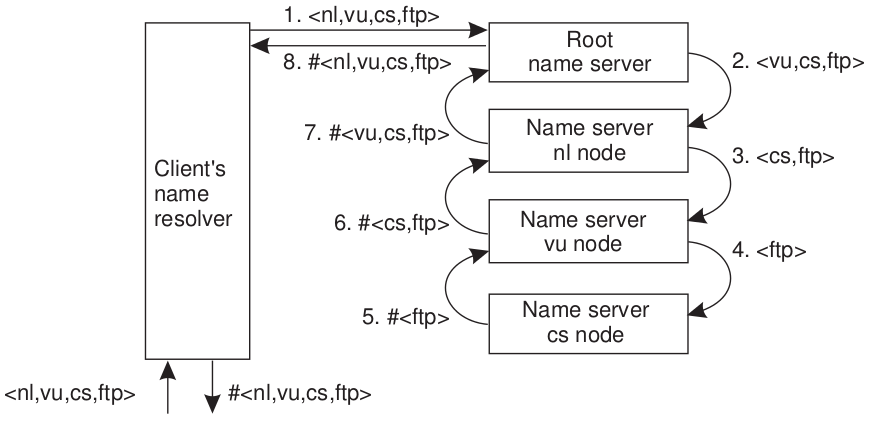
\includegraphics[scale=0.7]{recursiv}
\caption{Iterative request for an IP-address}
\label{fig:recursiv}
\end{figure}


\newpage
\section{DNS security extentions}\label{sec:DNS-security}
Due to security issues various governments, research organizations and others have developed a specification and associated protocol called DNS Security extensions (DNSSEC) which protects DNS querty/response transactions \cite[p. 84]{DNS-article}.

Two main security threats exist for DNS in the context of query/
response transactions. Attackers can

	\begin{itemize}%[ref=test]
	\item spoof authoritative name servers responding to DNS queries and alter DNS responses

	\item alter the DNS responses stored in caching name servers.
	\item[] \hspace{100mm}\cite[p. 84]{DNS-article}
	\end{itemize} 
DNSSEC was designed to protect the users from obtaining corrupted DNS data. 
It contains a set of extensions to DNS which provide origin authentication of DNS data, authenticated denial of existence, and data integrity.
If a DNS server uses DNSSEC it is marked as a \textit{signed zone}.



A signed zone is a DNS server zone which includes a digital signature for all content it returns.
It verifies that the underlying responses have requested resource records, special resource records that carry the digital signatures associated with the requested resources and it contains a DNSKey which include a public key which can verify the signature.



Using signed zones as authentication requires a DNSSEC-aware caching name server which start from a trusted public key stored within it self, a \textit{trust anchor}.
This establish a chain of trusted DNS servers with DNSSEC implemented to the public key of the zone. 
It is also possible to use a \textit{trust achor list} which contains a list over trusted anchors.

\end{document} 